\newpage
\section{SYSTEM DESIGN}

\subsection{System Overview}
The system uses initally predicts the personality of the user with the help of their social media account(facebook). Thus initially a classifier is to be trained to classify the personality of the user on the basis of their status update. Afterwards, the predicted personality of the user is to be used as one the metrics for the similar user computation in collaborative filtering and the effect of the personality on the colloaborative filtering engine was observed.

\subsection{System Architecture}
The give figure below is the architectural diagram of the project showing the process that are involved during the development of the project.

\begin{figure}[!ht]
\centering
\includegraphics[width = 16 cm]{fig/pbrs.png}
\caption{block diagram of the system}
\label{fig:project}
\end{figure}

\begin{itemize}
	\item Data Preprocessor: This subsystem is responsible for the conversion of the status update of the user from the dataset \cite{dataset} as well user logged in via api \cite{api} into vector representation via the use of bag of word and tf-idf model.\\
It is responsible for:
		\begin{enumerate}
			\item Lower casing the status update.
			\item Tokenization
			\item Filtering stop words
			\item Filtering parts of speech
			\item Stemming
			\item Conversion of textual data to vector respresentation(numerical form)
		\end{enumerate}
	\item Classifier: After the vector respresentation of the status update,this subsystem is responsible for personality prediction. Classifier are trained by the admin in the system using the dataset \cite{dataset} in order to predict a presonality. In the project there are three classifier model used for the personality classification.\\
They are:
\begin{enumerate}
	\item Naive Bayes Classifier
	\item Logistic Regression
	\item KNN 
\end{enumerate}
\item Recommender System: The system comprises of the eight models for the recommendation of the music to the user.\\
They are:
\begin{enumerate}
	\item Global Baseline Approach
	\item User to User collaborative filtering with rating matrix
	\item User to User collaborative filtering with personality matrix
	\item User to User collaborative filtering with weighted average of rating and personality matrix
	\item Combination of global baseline and CF with rating matrix
	\item Combination of global baseline and CF with personality matrix
	\item Combination of gloabal baseline and CF with weighted average of rating and personality matrix
	\item Matrix Factorization
\end{enumerate}
\item Storage Unit: It is reponsible for storing of user data, music data, user-music-rating data and user-music-recommendation data made by the recommender system. SQLite database is used as the storage unit for the project.
\end{itemize}

\newpage
\subsection{Use Case Diagram}
The use case diagram of the system depicting the actors and their interaction to the system is given in the figure below:
\begin{figure}[!ht]
\centering
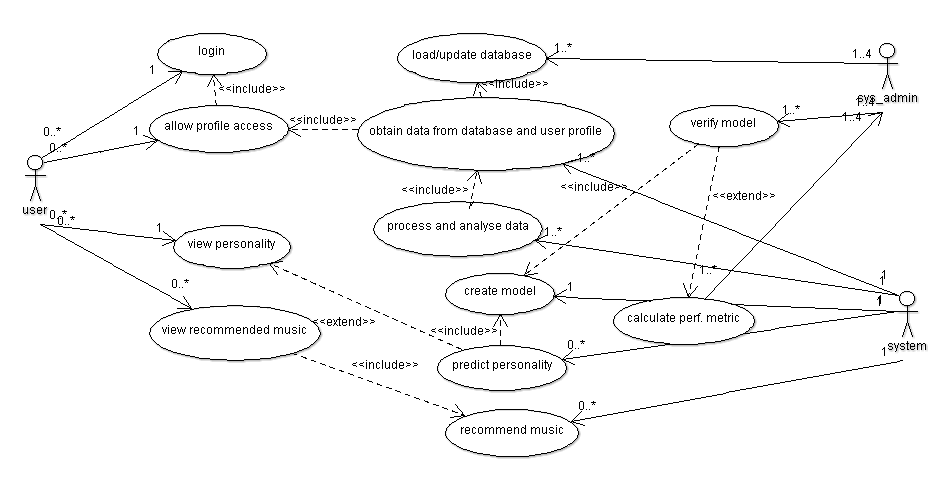
\includegraphics[width = 16 cm]{fig/Use.png}
\caption{Use Case Diagram of the System}
\label{fig:usecase}
\end{figure}

From the above diagram, it is clear that the system consists of two actors.They are:
\begin{itemize}
\item User: They are the ones who will be using the system directly. The users will be able to do the actions like login, viewing recommendation and listening to a music. 
\item Admin: Admin is directly responsible for training a classifier subsystem and recommender subsystem, creation of model for the storage engine and verification of all of these subsystem.
%\item Classifier: It is responsible for the classification of the personality of the user.
%\item Recommder System: It is responsible for the recommendation of the music to the user.
%\item Storage Handler: It is responsible for the creation of the data base model and storage of system data.
\end{itemize}

\newpage
\subsection{Class Diagram}
\begin{figure}[!ht]
\centering
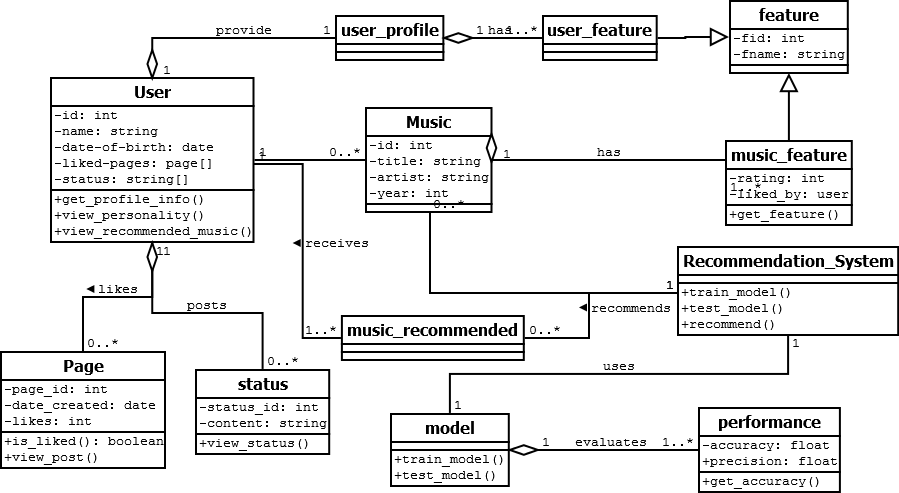
\includegraphics[width = 16 cm]{fig/class.png}
\caption{Class Diagram of the System}
\label{fig:class}
\end{figure}

\newpage
\subsection{ER Diagram}
The  ER diagram depicting the entities used in the system and relationship between them is given below:
\begin{figure}[!ht]
\centering
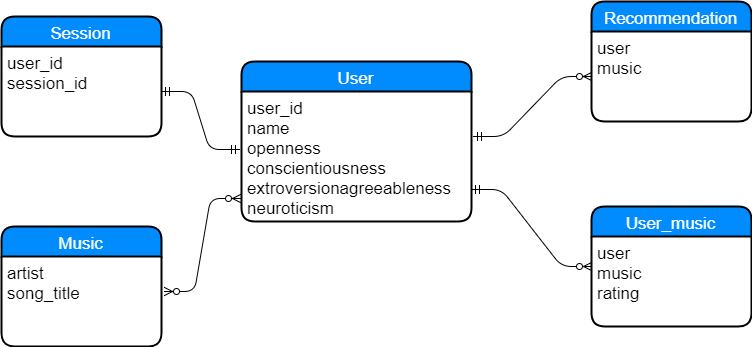
\includegraphics[width = 16 cm]{fig/erdiagram.png}
\caption{ER diagram of the System}
\label{fig:er}
\end{figure}
The entities in the system are:
\begin{enumerate}
	\item Session: It consists of attributes: session id and user id and has one to one relationship with user.
	\item Music: It consists of attributes: artist and songtitle and also has zero or many to zero or many relationship with the user-music. 
	\item User: It conists of attributes userid, name and personality traits attributes and has zero or many to zero or many relationship with user-music and recommendation and one to one with the session. 
	\item Recommendation: It consists of attributes user and music and has oone to one realationship with user while many to many realationship with music.
	
	\item User-Music: It consits of attributes user, music and rating and many to many relationship with user and music. 
\end{enumerate}
\newpage
\subsection{Activity Diagram}
\begin{figure}[!ht]
\centering
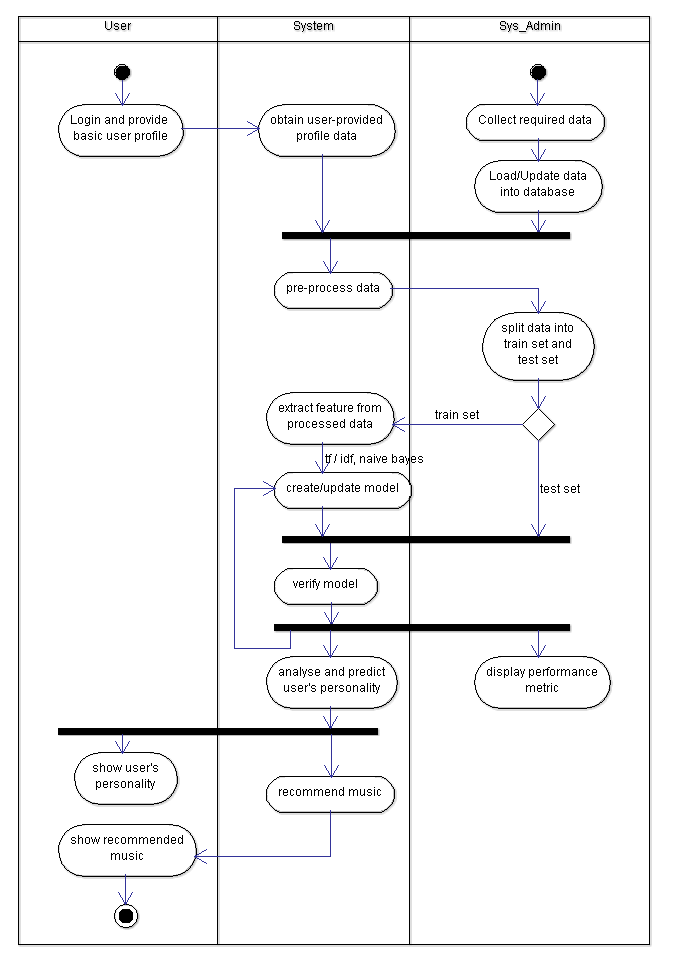
\includegraphics[width = 12 cm]{fig/Activity.png}
\caption{Activity Diagram of the System}
\label{fig:activity}
\end{figure}

\newpage
\subsection{Data Flow Diagram}
\begin{figure}[!ht]
\centering
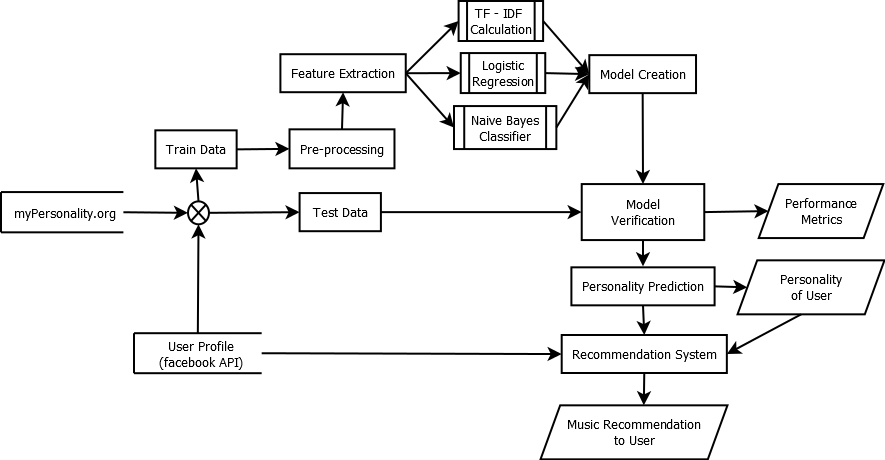
\includegraphics[width = 16 cm]{fig/System.png}
\caption{Data Flow Diagram of the System}
\label{fig:dfd}
\end{figure}
